\documentclass[aspectratio=169]{beamer}
% \documentclass[aspectratio=169,handout]{beamer}

\usetheme[titleformat=regular%
,numbering=fraction% use slide numbers
]{metropolis}
\metroset{%
  progressbar=foot,%
  %background=dark,
  block=fill
}
\only<handout>{\metroset{sectionpage=none}}
\only<handout>{\usecolortheme{dove}}
\usepackage{appendixnumberbeamer} % separate appendix
\usepackage[citestyle=authortitle,sorting=none]{biblatex}
\setbeamerfont{footnote}{size=\tiny}
\addbibresource{mae.bib}

% multimedia in beamer presentations
\usepackage{multimedia}

% adding some better facilities to latex such as proper booleans
\usepackage{etoolbox}

% Unicode math symbols for XeLaTeX
\usepackage{mathrsfs}

% standard math packages
\usepackage{amssymb}
\usepackage{amsthm}
\usepackage{amsmath}
\usepackage{amstext}
\usepackage{mathabx}
\usepackage{stmaryrd}
% math tools for amsmath
\usepackage{mathtools}

\usepackage{proof}

\usepackage{pgfpages}

\usepackage{listings}
\usepackage{xcolor}

% subfigures, subfloats
\usepackage{subcaption}

% for multiinclude
\usepackage{xmpmulti}

% tikz & friends

\usepackage{galois}
\usepackage{tikz}
\usetikzlibrary{fit,calc,shapes,arrows.meta,patterns,backgrounds}
\usetikzlibrary{decorations.pathmorphing}
\usetikzlibrary{cd}
\usetikzlibrary{positioning}
\usepackage[beamer]{hf-tikz}

% for author-title-year citing
\usepackage{xpatch}

\newcommand{\tikzmark}[1]{%
  \tikz[overlay,remember picture,baseline] \node [anchor=base] (#1) {};}

\newenvironment{tightcenter}{%
  \setlength\topsep{0pt}
  \setlength\parskip{0pt}
  \begin{center}
}{%
  \end{center}
}

% new colors
\definecolor{lightblue}{RGB}{217,220,253}
\definecolor{lightred}{RGB}{251,216,218}

\DeclareMathOperator{\pw}{\mathcal{P}} % powerset
\newcommand{\fset}[1]{\mathsf{#1}}
\newcommand{\nats}{\mathbb{N}}
\newcommand{\zahlen}{\mathbb{Z}}
\newcommand{\bools}{\mathbb{B}}
\newcommand{\Set}[1]{\left\{#1\right\}}
\newcommand{\true}{\kw{true}}
\newcommand{\false}{\kw{false}}
\newcommand{\sidenote}[1]{\hfill\quad \textsf{#1}}

\newcommand{\disunion}{+}

% named set
\newcommand{\ns}[1]{\mathit{#1}}
% function
\newcommand{\fn}[1]{\mathrm{#1}}
% "vector of"
\newcommand{\vo}[1]{\overrightarrow{#1}}
% "set of"
\newcommand{\setOf}[1]{\overline{#1}}
% syntactic tag
\newcommand{\sTag}[2]{\textsf{\textbf{#1}}\,#2}
% keyword
\newcommand{\kw}[1]{\texttt{#1}}
% usual suspects
\newcommand{\State}{\ns{State}}
\newcommand{\Value}{\ns{Value}}
\newcommand{\Stmt}{\ns{Stmt}}
\newcommand{\Env}{\ns{Env}}
\newcommand{\Store}{\ns{Store}}
\newcommand{\Kont}{\ns{Kont}}
% syntactic domains
\newcommand{\Exp}{\ns{Exp}}
\newcommand{\Var}{\ns{Var}}
\newcommand{\Addr}{\ns{Addr}}
% put a value to a pointer
\newcommand{\update}{\leftarrow}

% ebnf
\newcommand{\eDEF}{\,::=\;}
\newcommand{\eOR}{\;\vert\;}

\newcommand{\widen}{\nabla}

% \newcommand{\|}{\,\vert\,}

\newcommand{\todo}[1]{\iftoggle{TODO}{\textcolor{red}{TODO: #1}}{}}
% ceiling and floor symbols
\DeclarePairedDelimiter\ceil{\lceil}{\rceil}
\DeclarePairedDelimiter\floor{\lfloor}{\rfloor}

% big O notation
\DeclareMathOperator{\bigO}{O}

% fixed points
\DeclareMathOperator{\lfp}{lfp}

% print both years for bibliography
\renewbibmacro*{cite:labelyear+extrayear}{%
\iffieldundef{labelyear}
{}
{\printtext[bibhyperref]{%
\iffieldundef{origyear}{}{\printfield{origyear}\addslash}%   <--- added
\printfield{labelyear}%
\printfield{extrayear}}}}

\renewbibmacro*{date+extrayear}{%
\iffieldundef{year}
{}
{\printtext[parens]{%
\iffieldundef{origyear}{}{\printfield{origyear}\addslash}%  <--- added
\printdateextra}}}

% overlay an image
\def\Put(#1,#2)#3{\leavevmode\makebox(0,0){\put(#1,#2){#3}}}

% text over symbols nicely, requires amsmath for overset
\newcommand\textoverop[2]{\mathrel{\overset{\makebox[0pt]{\mbox{\normalfont\tiny\sffamily #1}}}{#2}}}

% special arrows
\newcommand\monarrow{\textoverop{mon}{\rightarrow}}

% theorems
\newtheorem{thm}{Theorem}
\newtheorem{eg}{Example}

\newcommand{\abscolor}[1]{\textcolor{mLightBrown}{#1}}
\newcommand{\concolor}[1]{\textcolor{mLightGreen}{#1}}
\newcommand{\abst}[1]{#1^{\#}}

\newcommand{\step}{\rightsquigarrow}

\newcommand{\altm}{\; {\color{black}\mid}\; }

% listings setup
%\lstset{basicstyle=\tiny\ttfamily,columns=fixed}

\usepackage{fnpct}
\AdaptNoteOpt\footcite\multfootcite

\xapptobibmacro{cite}{\setunit{\nametitledelim}\printfield{year}}{}{}

% highlighting lines in listings

% two approaches: https://tex.stackexchange.com/questions/8851/how-can-i-highlight-some-lines-from-source-code)
\lstset{
  basicstyle=\scriptsize\ttfamily,language=[LaTeX]Tex,breaklines=true,
  breakautoindent=true,breakindent=2ex,
}

\tikzset{onslide/.code args={<#1>#2}{%
  \only<#1>{\pgfkeysalso{#2}} % \pgfkeysalso doesn't change the path
}}

\makeatletter
\newenvironment<>{btHighlight}[1][]
{\begin{onlyenv}#2\begingroup\tikzset{bt@Highlight@par/.style={#1}}\begin{lrbox}{\@tempboxa}}
{\end{lrbox}\bt@HL@box[bt@Highlight@par]{\@tempboxa}\endgroup\end{onlyenv}}

\newcommand<>\btHL[1][]{%
  \only#2{\begin{btHighlight}[#1]\bgroup\aftergroup\bt@HL@endenv}%
}
\def\bt@HL@endenv{%
  \end{btHighlight}%   
  \egroup
}
\newcommand{\bt@HL@box}[2][]{%
  \tikz[#1]{%
    \pgfpathrectangle{\pgfpoint{1pt}{0pt}}{\pgfpoint{\wd #2}{\ht #2}}%
    \pgfusepath{use as bounding box}%
    \node[anchor=base west, fill=orange!30,outer sep=0pt,inner xsep=1pt, inner ysep=0pt, rounded corners=3pt, minimum height=\ht\strutbox+1pt,#1]{\raisebox{1pt}{\strut}\strut\usebox{#2}};
  }%
}
\makeatother

% more coloring in equations?
\newcommand{\colorIt}[3]{
   \tikz[baseline]{ \node[fill=#1!20,anchor=base,rounded corners=2pt] (#2) {\ensuremath{#3}};}
}

\usepackage{listings-rust}

%%% Local Variables:
%%% mode: latex
%%% TeX-master: "main"
%%% TeX-engine: xetex
%%% End:


\only<handout>{
  \pgfpagesuselayout{4 on 1}[letterpaper,border shrink=5mm,landscape]
}

\newtoggle{notes}
%\only<beamer>{\toggletrue{notes}}

% add notes:
\iftoggle{notes}{
  \makeatletter
  \def\beamer@framenotesbegin{% at beginning of slide
    %\gdef\beamer@noteitems{}%
    %\gdef\beamer@notes{}%
    \usebeamercolor[fg]{normal text}
  }
  \makeatother
  \setbeamertemplate{note page}[plain]
  \setbeamerfont{note page}{size=\footnotesize}
  \setbeameroption{show notes on second screen=right}
}{}

\newtoggle{labdemo}
%\toggletrue{labdemo}
\newtoggle{TODO}
\toggletrue{TODO}

\title[Major Area Exam]{Memory Safety in Systems Languages} %Techniques for
%\subtitle{Tradeoffs in Efficiency and Completeness}
%\subtitle{A Balancing Act}
\subtitle{Major Area Exam}
\date{June 11, 2018}
\author{Michael Christensen}
\institute[UCSB]{
  \normalsize
  {\large \bfseries Committee:}\\
  Ben Hardekopf (\,$\vcenter{\hbox{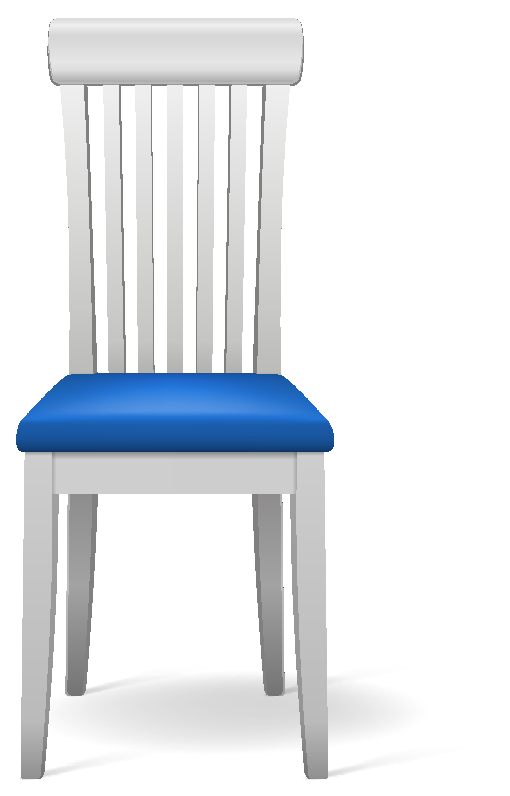
\includegraphics[height=1em]{chair/file.eps}}}$) \quad
  Tim Sherwood \quad
  Rich Wolski
}
\titlegraphic{\hfill\includegraphics[width=2.25cm]{ucsbseal_cmyk.pdf}}

\begin{document}
\maketitle

\metroset{numbering=none}
\begin{frame}<beamer>[noframenumbering]
  \frametitle{Outline}
  \tableofcontents
\end{frame}
\metroset{numbering=fraction}

\section{Motivation}
\begin{frame}{What is a System?}
Infrastructure software upon which applications are built
% (compilers, garbage collectors, file systems, drivers, etc.)
\\
    \vspace{0.2in}
\pause
Operating Systems
  \begin{itemize}[<+->]
          % need to be able to do this
    \item Process abstraction
    \item Named resource management
       \begin{itemize}
           \item Multiplex physical hardware resources
           \item Partition and abstract \textbf{memory}
       \end{itemize}
    \item Low overhead, robustness, security
  \end{itemize}
\end{frame}

%\notes{
% isolation third item for os
% files: hide peculiarites of disks/I/O decives, abstract model of device-indepdent files
% address space: virtual memory + protection
% process: running program container (registers, files, alarms, address space, etc.)
%}

\begin{frame}{Systems Languages}
\begin{itemize}[<+->]
    \item Past systems languages: \tiny{ALGOL, PL/I, Fortran, BCPL/B, C, Mesa/Cedar, Pascal/Modula-2/Oberon, C++, ...}
    \item C: the de-facto standard
        \begin{itemize}
            \item Data structure representation control
            \item Memory management control % don't need to use stdlib either
            \item Complete mutability via pointers % define what I mean here
            \item Performant
        \end{itemize}
    \item C: the unsafe standard
        \begin{itemize}
            \item Unchecked array operations $\Rightarrow$ buffer overflows
            \item Pointers $\equiv$ arrays $\Rightarrow$ hazardous pointer arithmetic
            \item Unsafe casts $\Rightarrow$ read/write arbitrary addresses
            \item Aliasing $\Rightarrow$ dangling pointers, double frees, null dereferences
        \end{itemize}
\end{itemize}
\end{frame}

%\notes{
% possibly add OS lang was used for, date
% ALGOL: formally defined syntax
% Mesa, Cedar: rich exceptions, GC
% Pascal (1971), Modula-2 (1982), Oberon (1988) % structured programming, records, pointers, dynamic allocation, information hiding, objects
% see mae3.org, mae4.org
%}

\begin{frame}{Memory Safety}
\begin{itemize}[<+->]
    \item Memory safety error: ``Any dereference of a pointer or subscripted array reference which reads or writes storage outside of the referent'' \footcite{austin_efficient_1994}
        \begin{itemize}
            \item Spatial: outside referent's \alert{address bounds}
            \item Temporal: outside referent's \alert{lifetime}
        \end{itemize}
    \item Ideal technique is
        \begin{itemize}
            \item Efficient and expressive % (hallmarks of C)
            \item Purely static % (no runtime overhead)
            \item Precise % (not overly conservative)
            \item Automatic % (legacy code $\Rightarrow$ no source or memory layout change)
        \end{itemize}
%    \item Non-goals: secrecy, security, concurrency, type safety % but are natural consequences of safety
    \item Memory errors become \alert{type errors}, management happens at \alert{compile-time}
\end{itemize}
\end{frame}

%\notes{
% some of those goals from nagakatte 201*
% undecidability of checking certain dynamic errors
% hard to verify/prove invariants about b/c
  % casts + pointers make c essentially untyped (rondon: type system is only to help know size of bytes to read/write)
  % aliasing
% make bad hard, useful easy
%}

\AtBeginSection[]
{
  \metroset{numbering=none}
  \begin{frame}<beamer>[noframenumbering]
    \frametitle{Outline}
    \tableofcontents[currentsection]
  \end{frame}
  \metroset{numbering=fraction}
}

\only<handout>{
  \addtocounter{framenumber}{1}
}

\section{Spatial Safety}

\begin{frame}[fragile]{Spatial Safety}
  \footnotesize
  \begin{columns}[T]
    \begin{column}{0.45\textwidth}
        Prevent accessing out of object's bounds
        \\
        Some approaches:
        \begin{itemize}
            \item Dynamic \footnotesize{(fat pointers, bounds tables, objects)}
            \item Semi-static \footnotesize{(constraint checking via annotations and dependent types})
        \end{itemize}
    \end{column}
    \begin{column}{0.45\textwidth}
\begin{lstlisting}[language=C,mathescape] %,basicstyle={\footnotesize\ttfamily}]

int sum(int *buf, int *end) {
    int sum = 0;
    while(buf < end) {
        sum += *buf;
        int *tmp = buf + 1;
        buf = tmp;
    }
    return sum;
}
\end{lstlisting}
Let's list the potential problems:
        \begin{itemize}
            \item $\texttt{buf}$ or $\texttt{end}$ could be null
            \item $\texttt{buf}$ and $\texttt{end}$ could be entirely unrelated
            \item $\texttt{buf}$ might not be an array % e.g. pointer to struct? problem with casting
        \end{itemize}
    \end{column}
  \end{columns}
\end{frame}

\subsection{Fat Pointers and Metadata}

\begin{frame}[fragile]{Fat Pointers}
  \footnotesize
Fat pointers
\begin{itemize}
 \item Contains metadata such as base address and bounds along with value
 \item Safe and quick to retrieve find metadata
 \item Incompatibility with uninstrumented libaries, run-time overhead, bloated code size
 \item Automatic run-time check insertion to overcome static detection weakness
 \item Approximately 3\% - 200\% runtime overhead versus plain
\end{itemize}
\end{frame}

\begin{frame}{Fat Pointers}
SafeC \footcite{austin_efficient_1994}:
  \begin{itemize}
     \item Compile-time transform, replace all pointers and extend all pointer definitions
     \item Fields include:
          \begin{itemize}
             \item base, size, storage class (errant deallocations)
             \item Unique capability issued to an allocation
          \end{itemize}
     \item Insert array access checks before each pointer/array dereference
     \item Complete spatial safety as long as
         \begin{itemize}
            \item transparent storage management
            \item no safe pointer object attribute manipulation
         \end{itemize}
     \item 275\% space overhead, 2-6x runtime overhead, 0.35-3x code size overhead
         \begin{itemize}
            \item safe pointers aren't register allocated
            \item compiler optimizations fail with additonal checks
         \end{itemize}
  \end{itemize}
\vspace{0.2in}
\end{frame}

\begin{frame}{Fat Pointers}
\footnotesize
CCured \footcite{necula_ccured:_2002}:
      \begin{itemize}
          \item Strong type system helps inference statically optimize different pointer uses % whole program type inference
          \item $\texttt{SAFE}$: almost no overhead, no ptr arith, array indexing, type casts
          \item $\texttt{SEQ}$: fat pointers allow arith, indexing, some casts
          \item $\texttt{WILD}$: arbitrary casts, expensive dynamic checks
%          \item Very detailed description of run-time checks generated and translation for each expression
          \item Relies on a garbage collector
          %\item 3\%-87\% runtime overhead increase
      \end{itemize}

Cyclone \footcite{jim_cyclone:_2002}: % offshoot of TAL/popcorn
      \begin{itemize}
          \item Array vs non-array pointers (never-null, fat, unitialized warning via control-flow analysis)
          \item Tagged unions and automatic tag injection (e.g. $\texttt{printf}$)
          %\item Statically validate and remove non-array fat pointers
          \item Arrays and strings converted automatically to fat
          %\item 40\% runtime overhead
          %\item Uses regions + automatic memory management for temporal safety (free is a no-op) (see nice example)
          %\item never null don't need checks, use @; push back null checks from uses to their sources
          %\item ? permits pointer arithmetic
          %\item Restrict arithmetic on regular pointers
          %\item parametric polymorphism, subtyping, static analysis to check for safety, adding run-time checks
      \end{itemize}
\vspace{0.2in}
\end{frame}

\begin{frame}{Fat Pointers}
Cuckoo \footcite{west_cuckoo:_2005}
      \begin{itemize}
          \item Store array size in memory before array dimensions's first element
          \item Name of an array is pointer to an \emph{array}, not first object
          \item Type system for preventing assignment of automatic objects into longer-lifetime pointers
          \item Wrap dynamic memory allocation (type homogeneous pool-based) % will explain later
          \item Forbid addition and subtraction expressions including pointer operands! % statically determining given pointer points to an array object is undecidable
        % compile-time checks if array bounds are constants, otherwise run-time checks
      \end{itemize}

\end{frame}

\begin{frame}[fragile]{Fat Pointers}
  \footnotesize
  \begin{columns}[T]
    \begin{column}{0.45\textwidth}
    $\vcenter{\hbox{\includegraphics[height=8em]{fig/FIGURE_necula-2005_ccured-seq.PNG}}}$
    \end{column}
    \begin{column}{0.45\textwidth}
\begin{lstlisting}[language=C,mathescape] %,basicstyle={\footnotesize\ttfamily}]

int sum(int *SEQ buf, int *SEQ end) {
    int sum = 0;
    while(buf < end) {
        assert(buf.b $\leq$ buf.p $\leq$ buf.e - sizeof(int));
        sum += *(buf.p);
        buf.p = buf.p + (1 * sizeof(int));
        buf.b = buf.b;
        buf.e = buf.e;
    }
    return sum;
}
\end{lstlisting}
    \end{column}
  \end{columns}
\end{frame}

%% - fullcite:akritidis_baggy_2009
%% - fullcite:brunink_boundless_2011

\begin{frame}[fragile]{Separate Metadata}
Avoid fat pointers by spltting bounds and base metadata
\\
MSCC \footcite{xu_efficient_2004}
    \begin{itemize}
        \item Shadow structures mirror entire original structure
        \item Checked pointers modified by external libraries must have metadata updated at the library call via wappers
        \item 1.63x overhead
    \end{itemize}
\end{frame}

\begin{frame}{Separate Metadata}
CCured (2005) \footcite{necula_ccured:_2005} % Note: improves original CCured work
    \begin{itemize}
        \item Reduce number of WILD pointers
            \begin{itemize}
                \item use physical subtyping for handling upcasts
                \item special pointer carrying runtime-type info for downcasts
            \end{itemize}
        \item Fix compatiblity issues
            \begin{itemize}
                \item specify conversions, checking at boundaries with precompiled libraries
                \item separate metadata in mirror data structure (perf hit b/c of loss of locality)
            \end{itemize}
    \end{itemize}
Softbound \footcite{nagarakatte_softbound:_2009}
    \begin{itemize}
        \item Insert runtime bounds checks, consulting disjoint metadata via table lookup
%        \item \todo{fix disjoint shadow data structure by ...}
        \item Handles arbitrary casts, sub-object overflows not covered by MSCC
        \item Transforms every func decl and call-site to pass base and bound arguments % for metadata propagation
    \end{itemize}
\vspace{0.2in}
\end{frame}

\begin{frame}{Separate Metadata}
Checked C \footcite{ruef_checked_2017}
    \begin{itemize}
        \item Extend C with two \emph{checked pointer types}, automatically rewrite code to use when possible
        \item Derefence-only (no arith.) pointer, Arithmetic-supporting (possibly null-terminated) pointer with bounds in type
%        \item $\verb{_Ptr<T>}$, a pointer for dereference only (no arith)
%        \item $\verb{_Array_ptr<T>}$ and $\verb{_Nt_array_ptr<T>_}$, supporting arith w/ bounds declarations in type (latter is null-terminated)
        \item Isolate (un)safe code with \emph{checked code regions} at file/func/block level; prevent unchecked pointer usage and certain casts
        \item Cannot blame checked code for violation
%       \item Compiler confirms restrictions maintained, inserts checks on ptr access
    \end{itemize}
\end{frame}


\begin{frame}[fragile]{Separate Metadata}
  \footnotesize
  \begin{lstlisting}[language=C,numbers=left,mathescape,basicstyle={\footnotesize\ttfamily}]
int sum(int *buf, int *end) {
    int sum = 0;
    $\colorbox{red!30}{int bufbase = table\_lookup(buf)->base;}$
    $\colorbox{red!30}{int bufbound = table\_lookup(buf)->bound;}$
    while(buf < end) {
        $\colorbox{red!30}{if ((buf < bufbase) || ((buf + sizeof(buf)) > bufbound)) abort;}$
        sum += *buf;
        int *tmp = buf + 1;
        $\colorbox{red!30}{int tmpbase = bufbase; int tmpbound = bufbound;}$ // inherit base and bound
        $\colorbox{red!30}{int bufbase = tmpbase; int bufbound = tmpbound;}$ // would be optimized out
        buf = tmp;
    }
    return sum;
}
  \end{lstlisting}
\end{frame}
% question: where is table stored (heap or stack?)

\subsection{Annotations and Dependent Types}
% annotations provided by user
% don't change memory layout
% prove as much statically as possible
% use run-time checks where static checking is not sufficient

\begin{frame}[fragile]{Extended Type Checking}
Extended Type Checking (ETC) \footcite{detlefs_overview_1995}
    \begin{itemize}
      \item use automatic theorem prover to detect index bounds in Modula-3
      \item use info in annotations to assist
      \item easier than C b/c no ptr arithmetic
    \end{itemize}
Also see: ETC/Java \footcite{flanagan_extended_2002}
\end{frame}

\begin{frame}[fragile]{LCLint}
LCLint \footcite{larochelle_statically_2001}
\begin{itemize}
    \item Leverage LCLint, an annotation-assisted buffer detection tool
    \item Annotations that constrain possible values a reference contains before/after funcall
    \item Function pre/post-condition with: \footnotesize{$\texttt{requires, ensures, unique, returned, modifies, out}$} clauses
    \item Assumptions are ~minSet~, ~maxSet~, ~minRead~, ~maxRead~
% TODO put notes of what these mean!!!
    \item Generates constraints at expression level, resolved w/ checking at statement level
    \item Heuristics to deal with loops nicely enough; neither sound nor complete
\end{itemize}
Also see: CSSV \footcite{dor_cssv:_2003}
    \vspace{0.2in}
\end{frame}
% \item gives decent examples of use

%\begin{frame}[fragile]{CSSV}
%CSSV \footcite{dor_cssv:_2003}
%\begin{itemize}
%    \item source-to-source translation
%    \item instruments program w/ additional variables describing string attrs
%    \item adds ~assert~ statements checking for unsafe string ops
%    \item statically analyze instr. version with *integer analysis* to determine possible assertion failures
%    \item handles overlapping ptrs, etc.
%    \item  disadv: \# vars in instr. quadratic in \# in orig.
%\end{itemize}
%\end{frame}

%- fullcite:bodik_abcd:_2002 <----
%- fullcite:wagner_first_2000 
%- disadv: proves correct fraction of array/ptr references (useful for reducing checks)

\begin{frame}[fragile]{Annotations}
  \footnotesize
  \begin{columns}[T]
    \begin{column}{0.45\textwidth}
        Foo bar baz
    \end{column}
    \begin{column}{0.45\textwidth}
%      \lstinputlisting[language=C,mathescape]{lst/spatial_objs.c}
       \begin{lstlisting}[language=C,numbers=left,mathescape,basicstyle={\footnotesize\ttfamily}]
int main() {
    printf("hello, world!\n");
}
$$
        \end{lstlisting}
    \end{column}
  \end{columns}
\end{frame}

\begin{frame}{Dependent Types}
    Dependent types are \emph{typed-valued functions} \footcite{pierce_advanced_2005}
    \begin{itemize}
        \item E.g. type family of vectors: $\texttt{Vector :: Nat}\rightarrow\texttt{*}$.
        \item Introduce with \emph{dependent product type}: $\texttt{vecnew : }\Pi\texttt{n:Nat.data}\rightarrow\texttt{Vector n}$.
        \item Combine as well: $\texttt{cons : }\Pi\texttt{n:Nat.data}\rightarrow\texttt{Vector n}\rightarrow\texttt{Vector(n+1)}$.
        \item Generalizes arrow type
        \item Based on type theory work by Martin-Lof \footcite{martin-lof_constructive_1984}
    \end{itemize}
\end{frame}

\begin{frame}{Dependent Types in Functional Languages}
\vspace{-0.1in}
Dependent ML \footcite{xi_eliminating_1998}
\begin{itemize}
    \item Reduce static array bound checking to constraint satisfiability
    \item Limit indices to linear integer and boolean expressions; compile-time decidable
\end{itemize}
Cayenne (Haskell-like) \footcite{augustsson_cayennelanguage_1998}
\begin{itemize}
    %\item First time \emph{full dependent} types in a PL % TODO say
    \item No restriction on expressions in types
    %\item Example typing a C-style $\texttt{printf}$ function where $\texttt{PrinftType}$ returns a type % TODO say
    \item Undecidability of arbitrary expression equivalence and thus type checking
\end{itemize}
$\text{Xanadu}_{0}^{\Pi,\Sigma}$ (C-like) \footcite{xi_imperative_2000}
\begin{itemize}
    \item Like DML, restrict index expressions in types to integer constraint domain
%    \item Defines what it means for a type to equal/coerce into another
    \item Programmer must supply state type in order to type conditionals and loops
\end{itemize}
    \vspace{0.2in}
\end{frame}

% \item Allows trusted cast mechanism to supress errors

\begin{frame}{Dependent Types in Imperative Languages}
SafeDrive \footcite{zhou_safedrive:_2006} and Deputy \footcite{condit_dependent_2007}
    \begin{itemize}
        \item User-added annotations relating pointers to bounds
        \item Expressions in types limited to local variables, constants, and arithmetic expr
        \item Three phase pass over annotated C programs, emits C code
            \begin{itemize}
                \item Automatic bound variables addition
                \item Flow-insensitive type checking (insert run-time checks)
                \item Flow-sensitive check optimization
            \end{itemize}
    \end{itemize}
\vspace{-0.3in}

% here I need to exaplin what a grammer is for them
% TODO make an animation with colors describing things I talk about as I do
\footnotesize{
\begin{gather*}
    x,y \in \text{Variables}
    \quad
    \text{op} \in \text{Binary ops}
    \quad
    n \in \text{Integers}
    \quad
    \text{comp} \in \text{Comparison Ops}
\end{gather*}

\vspace{-0.3in}

\begin{columns}[T]
\begin{column}{0.45\textwidth}
\begin{alignat*}{2}
\text{Ctors}\quad &C &&::= \text{int} \altm \text{ref} \altm ...
\\
\text{Types}\quad &\tau &&::= C \altm \tau_1 \ \tau_2 \altm \tau\ e
\\
\text{Kinds}\quad & \kappa &&::= \text{type} \altm \text{type} \rightarrow \kappa \altm \tau \rightarrow \kappa
\\
\text{L-exprs} \quad &l &&::= x \altm *e
\end{alignat*}
\end{column}

\begin{column}{0.45\textwidth}
\begin{alignat*}{2}
\textit{Exprs}\quad &e &&::= n \altm l \altm e_1 \text{ op } e_2
\\
\textit{Cmds}\quad &c &&::= \text{skip} \altm c_1;c_2 \altm l := e \altm \text{assert}(\gamma) \altm
\\
~ & ~ && \text{let } x : \tau = e \text { in } c \altm \text{let } x = \text{new } \tau(e) \text{ in } c
\\
\text{Preds}\quad &\gamma &&::= e_1 \text{ comp } e_2 \altm \text{true} \altm \gamma_1 \wedge \gamma_2
\end{alignat*}
\end{column}
\end{columns}
}

\vspace{0.1in}

\end{frame}
%\note{
% kind of int is "type"
% kind of ref is "type -> type"
% loops, conditionals omitted for flow-insenstivei type system
% Types restricted to only contain expressions using constatns, local variables, arbitrary arithmetic operators
% Type environment is a predicate on the state of the program
%}

\begin{frame}{Deputy}
Judgments for checking the well-formedness of types, local expressions, predicated expressions, and commands

\pause

\begin{center}
\begin{tabular}{c}
\infer[(\textsc{var\ write})]
{\Gamma \vdash x \coloneqq e \Rightarrow \text{assert}(\bigwedge_{y \in \text{Dom}(\Gamma)}\gamma_y);\ x \coloneqq e }
{x \in \text{Dom}(\Gamma) \qquad
 \text{for\ all}(y:\tau_y) \in \Gamma,\ \Gamma \vdash y[e/x]:\tau_y[e/x] \Rightarrow \gamma_y }
\end{tabular}

\pause

\begin{tabular}{c}
\infer[(\textsc{array\ deref})]
{\Gamma \vdash *e; \tau \Rightarrow \gamma_e \wedge (0 < e_{len})}
{\Gamma \vdash e: \text{array } \tau \ e_{len} \Rightarrow \gamma_e}
\end{tabular}

\pause

\begin{tabular}{c}
\infer[(\textsc{array\ arith})]
{\Gamma \vdash e + e': \text{array } \tau\ (e_{len} - e') \Rightarrow \gamma_e \wedge \gamma_e' \wedge (0 \leq e' \leq e_{len})}
    {\Gamma \vdash e: \text{array } \tau\ e_{len} \Rightarrow \gamma_e
    \quad \Gamma \vdash e':\text{int} \Rightarrow \gamma_{e'}}
\end{tabular} 
\end{center}

\end{frame}
% var-write is a key contribution of type system
% $\textsc{var\ write}$ rule responsible for updates to variables in presence of dependent type variables, verifying assignment does not break any dependencies in current scope
% For example, we can add rules for arrays:
% also permits a coercion judgement for allowing an array to be used where a smaller one is expected

\begin{frame}
    \todo{describe how they use assertions afterwards}
\end{frame}

\begin{frame}{Deputy}
Support in C
    \begin{itemize}
        \item Generalize array constructor to possibly-null bounded pointer: \emph{$\text{ptr }\tau \ lo\ hi$}
            \begin{itemize}
                \item C-style pointer arithmetic via $\oplus$ operator
                \item $x:\text{ptr int } b\ (b \oplus 8)$ $\texttt{// 8 integer area starting at b}$
                \item $x:\text{ptr int } x\ (x \oplus n)$ $\texttt{// n integer area starting at x}$
                \item $x:\text{ptr int } x\ e\ \ \ \ \ \ \ \ $ $\texttt{// from x to e}$
            \end{itemize}
        \item Dependent untion tags
            \begin{itemize}
                \item Leverage C idiom: ``tag'' indicates union field in use
                \item Specify the condition for each union field to be usable
                \item \emph{$\text{union}_n\ \tau_1\ ...\ \tau_n\ e_1\ ...\ e_n$}
                \item $x:\text{struct }\{ tag:\text{int}\;\ u: \text{union}_2 \text{ int (ref int)} \ (\textit{tag} \geq 2)\ (\textit{tag} = 1) \}$
            \end{itemize}
    \end{itemize}
\end{frame}

\begin{frame}[fragile]{Deputy}
\begin{columns}[T]
\begin{column}{0.45\textwidth}
\begin{lstlisting}[language=C,mathescape] %,basicstyle={\footnotesize\ttfamily}]

int sum(int *  $\colorbox{green!30}{count(end - buf)}$ buf, int * end) {
    int sum = 0;
    while(buf < end) {
        sum += *buf;
        int *tmp = buf + 1;
        buf = tmp;
    }
    return sum;
}
\end{lstlisting}
\end{column}

\begin{column}{0.45\textwidth}
%      \lstinputlisting[language=C,mathescape]{lst/deputy_after.c}
\begin{lstlisting}[language=C,mathescape] %,basicstyle={\footnotesize\ttfamily}]

int sum(int *  $\colorbox{green!30}{count(end - buf)}$ buf, int * end) {
    int sum = 0;
    while(buf < end) {
        $\colorbox{red!30}{assert(0 < end - buf);}$
        sum += *buf;
        $\colorbox{blue!30}{int tmplen = (end - buf) - 1;}$
        $\colorbox{red!30}{assert(0 <= 1 <= end - buf);}$
        int * $\colorbox{blue!30}{count(tmplen)}$ tmp = buf + 1;
        $\colorbox{red!30}{(0 <= end - tmp <= tmplen);}$
        buf = tmp;
    }
    return sum;
}
\end{lstlisting}
\end{column}
\end{columns}
    \tiny{$\colorbox{green!30}{Programmer-supplied annotation}$}
    \\
    \tiny{$\colorbox{blue!30}{Code added during automatic dependency inference}$}
    \\
    \tiny{$\colorbox{red!30}{Assertions added during checking}$}
\end{frame}
% All checks here would be eliminated.

\begin{frame}{Dependent Types in Imperative Languages}
Low-Level Liquid Types \footcite{rondon_liquid_2008}, \footcite{rondon_low-level_2010}
\begin{itemize}
    \item Refinement types where predicates are conjunctions over qualifiers
    \item Functions qualified over locations they operate on
    \item Deal with collections using \emph{location folding} for checking out a copy to do strong updates on
\end{itemize}
Tyr \footcite{de_araujo_tyr:_2016}
\begin{itemize}
    \item Augments LLVM IR with dependent pointer types
    \item Uses programmer annotations insert run-time bounds checks
    \item LLVM optimizations remove always-true checks; error if always-false
\end{itemize}
\vspace{0.2in}
\end{frame}

\begin{frame}{A Hybrid Approach}
Low* \footcite{protzenko_verified_2017}
\begin{itemize}
    \item DSL for verified, efficient low-level programming in F* %(ML-like language with dependent types)
    \item Goal: write efficient \& verified C in a high-level language
    \item Write F* syntax against library modelling lower-level view of C memory
    \item Model arrays by implementation abstract buffer type using references by hyper-stacks % TODO define hyperstacks
    \item Translate Low* to CompCert Clight
\end{itemize}
\end{frame}

%\begin{frame}{An Overview of Spatial Safety Approaches}
%Several deficiencies
%\begin{itemize}
%  \item High runtime overhead
%  \item Incomplete detection of spatial violations
%  \item Incompatible pointer representations (changing memory layout)
%  \item  Non-trivial changes to source code
%  \item Whole program analyses (for low-overhead) [e.g. Dhurjati 2006, Necula 2005]
%  \item Some of these aren't complete or sound
%  \item  Completely detecting buffer overflow (i.e. bounds) in general is undecidable!
%\end{itemize}
%\end{frame}

\section{Temporal Safety}

\begin{frame}[fragile]{Temporal Safety}
  \footnotesize
  \begin{columns}[T]
    \begin{column}{0.45\textwidth}
        Prevent accessing object that has been \emph{previously deallocated}
        \\
        Some approaches:
        \begin{itemize}
            \item Effects and regions
            \item Unique pointers and linear types
            \item Ownership and borrowing
        \end{itemize}
    \end{column}
    \begin{column}{0.45\textwidth}
\begin{lstlisting}[language=C,mathescape] %,basicstyle={\footnotesize\ttfamily}]

int TODO() {
    // fill me in
}
\end{lstlisting}
Let's list the potential problems:
        \begin{itemize}
            \item Foo
            \item Bar
            \item Baz
        \end{itemize}
    \end{column}
  \end{columns}
\end{frame}

\begin{frame}{A Comment on Garbage Collection}
Garbage collection
    \begin{itemize}
        \item Relinquish control of location and layout of objects to runtime
        \item Non-zero overhead
        \item Complete temporal safety
        \item Sub-par memory use (time between unreachable and reclaimed)
        \item Used by several of the spatial approaches previously listed
        \item CCured etc. uses Boehm-Demers-Weister \footcite{boehm_garbage_1988} (free is no-op)
    \end{itemize}
\end{frame}
% \footcite{austin_efficient_1994}
% \footcite{jones_backwards-compatible_1997}
% \footcite{xu_efficient_2004}

\subsection{Effects and Regions}

\begin{frame}{Effects}
    Effect types describe the \emph{effects} of the computation leading to a value \footcite{pierce_advanced_2005}
    \\
    \todo{show simple very simple example}
\end{frame}

\begin{frame}{Effects}
    Fluent Languages \footcite{gifford_integrating_1986}
  \begin{columns}[T]
    \begin{column}{0.45\textwidth}
        \begin{itemize}
            \item Mix functional and imperative languages
            \item Every expression has a \emph{effect class}, restricting which subroutines or sublanguage features it may use
            \item Identify memoizable (referrentially transparent) expresions via a side effect lattice % for concurrency
        \end{itemize}
    \end{column}

    \begin{column}{0.45\textwidth}
    \footnotesize{
    \begin{tikzpicture}
      \node (WRA) at (0,3) {$\{W\ (R)\ (A)\}$};
      \node (RA)  at (0,2) {$\{R\ (A)\}$};
      \node (A)   at (0,1) {$\{A\}$};
      \node (e)   at (0,0) {$\{\}$};
      \draw (e) -- (A) -- (RA) -- (WRA);
    \end{tikzpicture}
        \begin{itemize}
            \item (W, WR, WA, WRA): "Procedure" class
            \item (R, RA): "Observer" class
            \item (A): "Function" class
            \item $\{\}$: "Pure" class.
        \end{itemize}
    }
    \end{column}
  \end{columns}
    See also: MFX \footcite{lucassen_polymorphic_1988}
\end{frame}

% note{
% mfx language, extends work using:
%   effect classes
%   full abstraction over effects
%   unmaskable side-effects
%   soundness proof
% }

\begin{frame}{Effects}
    Nielson and Nielson \footcite{nielson_type_1999} extend the simply-typed lambda calculus with annotations to demonstrate various forms of analyses:
    \begin{itemize}
        \item Control-Flow Analysis: annotate function types with function names used
        \item Binding Time Analysis: distinguish between dynamic and static data
        \item Side Effect Analysis:
            \begin{itemize}
                \item Reference variable represented by set of points where it could have been created (``region'')
                \item Annotate functions with actions they take (access, assignment, creation)
            \end{itemize}
        \item Region Inference: Compile-time determination of when to allocate regions, in which to allocate data
    \end{itemize}
\end{frame}

% BitC \footcite{shapiro_origins_2008} % a retrospective on BitC, what they were looking for (not too interesting)

\begin{frame}{Region-Based Memory Managememt}
    Regions \footcite{tofte_region-based_1997}
    \begin{itemize}
        \item Divide heap into sub-heaps (``regions'')
        \item Each region is like an unbounded stack, growing upwards
        \item \emph{Entire} region popped off region stack (no individual object deallocation)
        \item Explicit region polymorphism % regions can be given as arguments to functions at runtime
        \item Novelty: sound type system and region inference; analysis automatically identifies:
            \vspace{-0.1in}
            \begin{itemize}
                \item points where entire regions are allocated and deallocated
                \item into which region values should go
            \end{itemize}
        \item Used in ML Kit
        \item Disadvantage: unreasonable object lifetimes %(lifetime of expression must coincide with time takes to execute some subexpression)
    \end{itemize}
\end{frame}

\begin{frame}{Regions in C}
    Cyclone\footcite{grossman_region-based_2002}, again!
    \begin{itemize}[<+->]
        \item Three region types: single heap region (lives forever), stack regions (local-declaration blocks), dynamic regions (lexically-scoped lifetimes)
        \item Region-polymorphic functions
        \item Annotate pointers with regions into which they point; must be live for dereference
        \item Subtyping on lifetimes: can use region A where a region B is expected if A \emph{outlives} (is a subtype of) B
        \item Can specify partial orders on region lifetimes between pointers
        \item Type system for tracking capability (set of live regions) when dereferencing a pointer % no closures, but existential types can hide pointers to escape scope of their regions
        \item Sane defaults: infer region annotations on pointer types  % intraprocedural analysis => need function prototypes
        \item Static operator $\texttt{regions\_of}$ instead of effect variables
    \end{itemize}
    \vspace{0.1in}
\end{frame}

% TODO make an animation with colors describing things I talk about as I do
\begin{frame}{Cyclone}
\scriptsize{
\begin{alignat*}{2}
\text{kinds}\quad &\kappa &&::= T \altm R
\\
\text{type and region vars}\quad &\alpha,\rho &&
\\
\text{region sets}\quad &\epsilon &&::= \alpha_1 \cup ... \cup \alpha_n \cup \{\rho_1,...,\rho_m\}
\\
\text{region constraints} \quad &\gamma &&::= \emptyset \altm \gamma, \epsilon <: \rho
\\
\text{constructors} \quad &\tau &&::= \alpha \altm \text{int} \altm \tau_1 \xrightarrow[]{\epsilon} \tau_2 \altm \tau_1 \times \tau_2 \altm \tau \ast \rho \altm
\\
~ & ~ && \qquad \text{handle}(\rho) \altm \forall\alpha:\kappa \triangleright \gamma.\tau \altm \exists \alpha:\kappa \triangleright \gamma.\tau
\\
\text{expressions} \quad &e &&::= x_\rho \altm v \altm e\ \langle\tau\rangle \altm (e_1,e_2) \altm e.i \altm \ast e \altm \textbf{rnew}(e_1)e_2 \altm
\\
~ & ~ && \qquad e_1(e_2) \altm \&e \altm e_1 = e_2 \altm \textbf{pack} [\tau_1, e]\textbf{ as } \tau_1
\\
\text{values} \qquad &v &&::= i \altm f \altm \&p \altm \textbf{region}(\rho) \altm (v_1, v_2) \altm \textbf{pack}[\tau_1,v]\textbf{ as } \tau_2
\\
\text{paths} \qquad &p &&::= x_\rho \altm p.i
\\
\text{functions} \qquad &f &&::= \rho:(\tau_1\ x_{\rho}) \xrightarrow[]{\epsilon} = \{s\} \altm \Lambda\alpha:\kappa \triangleright \gamma.f
\\
\text{statements} \qquad &s &&::= e \altm \textbf{return } e \altm s_1;s_2 \altm \textbf{if } (e)\ s_1 \textbf{ else } s_2 \altm \textbf{while } (e)\ s \altm
\\
~ & ~ && \qquad \rho:\{\tau\ x_\rho = e;\ s\} \altm \textbf{region}\langle\rho\rangle\ x_{\rho}\ s \altm \rho:\{\textbf{open}[\alpha,x_{\rho}] = e;\ s\} \altm s\ \textbf{pop}[\rho]
\end{alignat*}
    }
\end{frame}

\begin{frame}{Example Cyclone Judgments}
$\Delta;\Gamma;\gamma;\epsilon;\tau \vdash_{stmt} s$
% Delta holds type and region variables in scope
% Gamma holds value variables in scope and types
% \gamma records partial order constraints relating region lifetimes
% \epsilon records capability (which regions in \Delta are live)
% tau is type e must have in any statement of form return e

% expressions access memory can be proven to be live from epsilon and gamma
\begin{center}
\begin{tabular}{c}
\infer[\textsc{var})]
{\Delta;\Gamma;\gamma;\epsilon \vdash x_\rho : \Gamma(x_\rho)}
{\gamma \vdash \Rightarrow \rho}
\end{tabular}

\pause
\vspace{0.1in}

\begin{tabular}{c}
\infer[(\textsc{deref})]
{\Delta;\Gamma;\gamma;\epsilon \vdash \ast e:\tau}
{\Delta;\Gamma;\gamma;\epsilon \vdash e:\tau \ast \rho \qquad \gamma \vdash \Rightarrow \rho}
\end{tabular}

\pause
\vspace{0.1in}

% every alpha and rho in epsilon_1 can be proven live from epsilon and gamma
\begin{tabular}{c}
\infer[(\textsc{call})]
{\Delta;\Gamma;\gamma;\epsilon \vdash e_1(e_2):\tau}
{\Delta;\Gamma;\gamma;\epsilon \vdash e_1 : \tau_2 \xrightarrow[]{\epsilon_1} \tau
    \qquad
 \Delta;\Gamma;\gamma;\epsilon \vdash e_2 : \tau_2 
    \qquad
 \gamma \vdash \epsilon \Rightarrow \epsilon_1}
\end{tabular}

\pause
\vspace{0.1in}

% type instantiation
\begin{tabular}{c}
\infer[(\textsc{type-inst})]
{\Delta;\Gamma;\gamma;\epsilon \vdash e\langle\tau_1\rangle: \tau_2[\tau_1 / \alpha]}
{\Delta;\Gamma;\gamma;\epsilon \vdash e : \forall\alpha:\kappa\triangleright\gamma_1 . \tau_2
    \qquad
 \Delta \vdash \tau : \kappa
    \qquad
 \gamma \vdash \gamma_1[\tau_1 / \alpha]}
\end{tabular}

% TODO review this
% novelty: ensuring gamma establishes constraints \gamma_1 used when type-checking e
% judgement \gamma \vdash \gamma' means for every \epsilon <: \rho in \gamma', we can show \gamma \vdash \rightarrow \epsilon
% \tau_2[\tau_2/alpha] is capture-avoiding substitution of \tau_1 for \alpha in \tau
% \gamma_1[\tau_1/alpha] is substitution of regions_of(\tau_1) for \alpha in \gamma_1

\end{center}
\end{frame}

\begin{frame}{Cyclone Example}
\todo{add example code}
\end{frame}

% TODO add frame on results, anything novel they should know
\begin{frame}{Cyclone Results}
Soundness Theorem:
    \begin{itemize}
        \item If starting statement is well-formed with respect to initial heap, the program cannot get stuck from type errors or dangling-pointer dereferences. 
        \item If program terminates, all regions it allocated will have been freed
    \end{itemize}
    % TODO it says GC can be used, but why?! what is it used for (pag 289)
Benchmarks
    \begin{itemize}
        \item Porting changes (mostly changing pointers to safe)
        \item 124 region-related changes (6\% of total) across 18,000 lines
        \item Near-zero overhead on non-compute intensive benchmarks % TODO why
    \end{itemize}
\end{frame}

\begin{frame}{More Regions}
    \footnotesize{
RC \footcite{gay_language_2001}
    \vspace{-0.1in}
   \begin{itemize}
     \item Fix region-related dangling pointers % aliasing!
     \item For each region, maintain a reference count of \# of external pointers pointing to objects in region % deleteregion fails if count is zero
     \item Type system + annotations ($\texttt{sameregion}, \texttt{traditional}, \texttt{parentptr}$) to help compiler remove annotation operations % no updating associated region % enforced by runtime checks
     \item Restrict C by disallowing arbitrary integer-to-pointer casts
     \item Cyclic data structures allowed (crossing cycles must break before deleting regions)
     \item No memory safey guarantee
% \item 27%-11% overhead
% TODO comment on the safety
   \end{itemize}
Reaps \footcite{berger_reconsidering_2002}
    \vspace{-0.1in}
   \begin{itemize}
     \item Combine regions and heaps into ``reaps''
     \item Behave like regions until $\texttt{reapFree}$ deallocates individual object
     \item Place freed object on a heap; subsequent allocations use heap until exhausted
%     \item Use Lea allocator generally, unless you need fast regions (i.e. reaps) % what their study found
   \end{itemize}
}
    \vspace{0.2in}
\end{frame}

\begin{frame}{More Regions/Effects}
Typestate \footcite{strom_typestate:_1986} %\item TODO add few more notes Determine subset of operations permitted in a particular context
\\
Vault \footcite{deline_enforcing_2001} % TODO review this
    \begin{itemize}
        \item Keys for representing run-time resources, held-key set, type guards
        \item Functions annotated with effect clause (pre- and post-conditions on held-key set contents)
        \item Freed regions before leaving scope
        \item Types enforce code must free a region
        \item Restrict aliasing, tracks fine-grained effects (requires more annotations)
        \item Catches Windows 2000 locking errors, I/O Request Packets ownership model corresponds to tracked types
        % todo add example?
    \end{itemize}
\end{frame}

\subsection{Linear Types and Ownership}

% introduce
\begin{frame}{Linear Types}
    \begin{itemize}
        \item \footcite{girard_linear_1987}
        \item \footcite{wadler_linear_1990}
        \item \footcite{kobayashi_quasi-linear_1999}
    \end{itemize}
\end{frame}

\begin{frame}{Applications}
    \begin{itemize}
        \item \footcite{ennals_linear_2004}: packet processing
        \item \footcite{hawblitzel_low-level_2004}: 
        \item \footcite{tov_practical_2011}
    \end{itemize}
\end{frame}

\begin{frame}{Cogent}
    \begin{itemize}
        \item \footcite{amani_cogent:_2016}
        \item \footcite{oconnor_cogent:_2016}
    \end{itemize}
\end{frame}

\begin{frame}{Ownership}
    \begin{itemize}
        \item \footcite{clarke_ownership_1998}
        \item \footcite{boyapati_ownership_2002}
        \item \footcite{fahndrich_language_2006}
        \item \footcite{smith_alias_2000}
        \item \footcite{matsakis_rust_2014}
        \item \footcite{levy_ownership_2015}
        \item \footcite{jung_rustbelt:_2017}
    \end{itemize}
\end{frame}

%\subsection{Extra Slides}

% TODO would be nice to mention since its modern stuff
%\begin{frame}{Other}
%    - Control-C
%    \footcite{fullcite:kowshik_ensuring_2002} <---------- (at least in passing)
%    \footcite{fullcite:dhurjati_memory_2003}
%    \footcite{kedia_simple_2017}
%        -adding manual memory amangement to high-level langauges C#/java
%    \item \footcite{petersen_type_2003}
%        - how to represent memory layout
%    \item \footcite{evans_static_1996} % talk about next to rust (See my notes): deal with problems in LCLint memory management
%\end{frame}

%\begin{frame}{Hardware and Other Support for Spatial Safety}
%\begin{itemize}
%    \item \footcite{arora_architectural_2006}
%    \item \footcite{devietti_hardbound:_2008}
%    \item \footcite{binary compatible, low overhead}
%      % - can reduce overhead of CCured's SEQ and WILD pointers, array bounds checking in C#
%    \item \footcite{cowan_stackguard:_1998}
%     % - inserts canaries
%    \item \footcite{hasabnis_light-weight_2012}
%     % - guard zones with good performance
%\end{itemize}
%\end{frame}

\end{document}

%%% Local Variables:
%%% mode: latex
%%% TeX-master: t
%%% TeX-engine: xetex
%%% End:
